\begin{algorithm}
	\caption{Lai ghép giữa các sinh vật được giữ lại}
	\begin{algorithmic}[1]
		\Require Danh sách sinh vật được giữ lại $kept\_creatures$, độ dài ADN $adn\_length$, chỉ số bị loại $removed\_idx$, thế hệ hiện tại $generation$
		\Ensure Sinh vật con mới được tạo từ phép lai ghép
		\State Chọn ngẫu nhiên $parent1$ từ $kept\_creatures$
		\State Chọn ngẫu nhiên $parent2$ từ $kept\_creatures$
		\State $k \gets$ Số nguyên ngẫu nhiên trong khoảng $[0, adn\_length - 1]$
		\State $adn \gets parent1.adn()[0:k] + parent2.adn()[k:adn\_length]$
		\State Tạo sinh vật con $child$ với ID $removed\_idx$, thế hệ $generation + 1$, ADN $adn$
		\State Thêm $parent1.id$ vào danh sách tổ tiên của $child$
		\State Thêm $parent2.id$ vào danh sách tổ tiên của $child$
		\State \Return $child$
	\end{algorithmic}
\end{algorithm}

\begin{algorithm}
	\caption{Đột biến quần thể sinh vật}
	\begin{algorithmic}[1]
		\Require Danh sách sinh vật $creatures$, tỷ lệ đột biến $mutation\_rate$, độ dài ADN $adn\_length$
		\Ensure Quần thể sinh vật sau khi đột biến
		\State $population \gets$ độ dài của $creatures$
		\State $mutated\_length \gets mutation\_rate \times population$
		\State $mutated\_creatures \gets$ Chọn ngẫu nhiên $mutated\_length$ sinh vật từ $creatures$
		\For{\textbf{each} $creature$ \textbf{in} $mutated\_creatures$}
		\State $gene\_index \gets$ Số nguyên ngẫu nhiên trong khoảng $[0, adn\_length - 1]$
		\State $value \gets$ Số thực ngẫu nhiên trong khoảng $[-1, 1]$
		\State $adn \gets creature.adn()$
		\State $adn[gene\_index] \gets value$
		\State $creature.update\_adn(adn)$
		\State $creature.mutated\_position.append(gene\_index)$
		\EndFor
		\State \Return $creatures$
	\end{algorithmic}
\end{algorithm}

\begin{figure}[h]
	\centering
	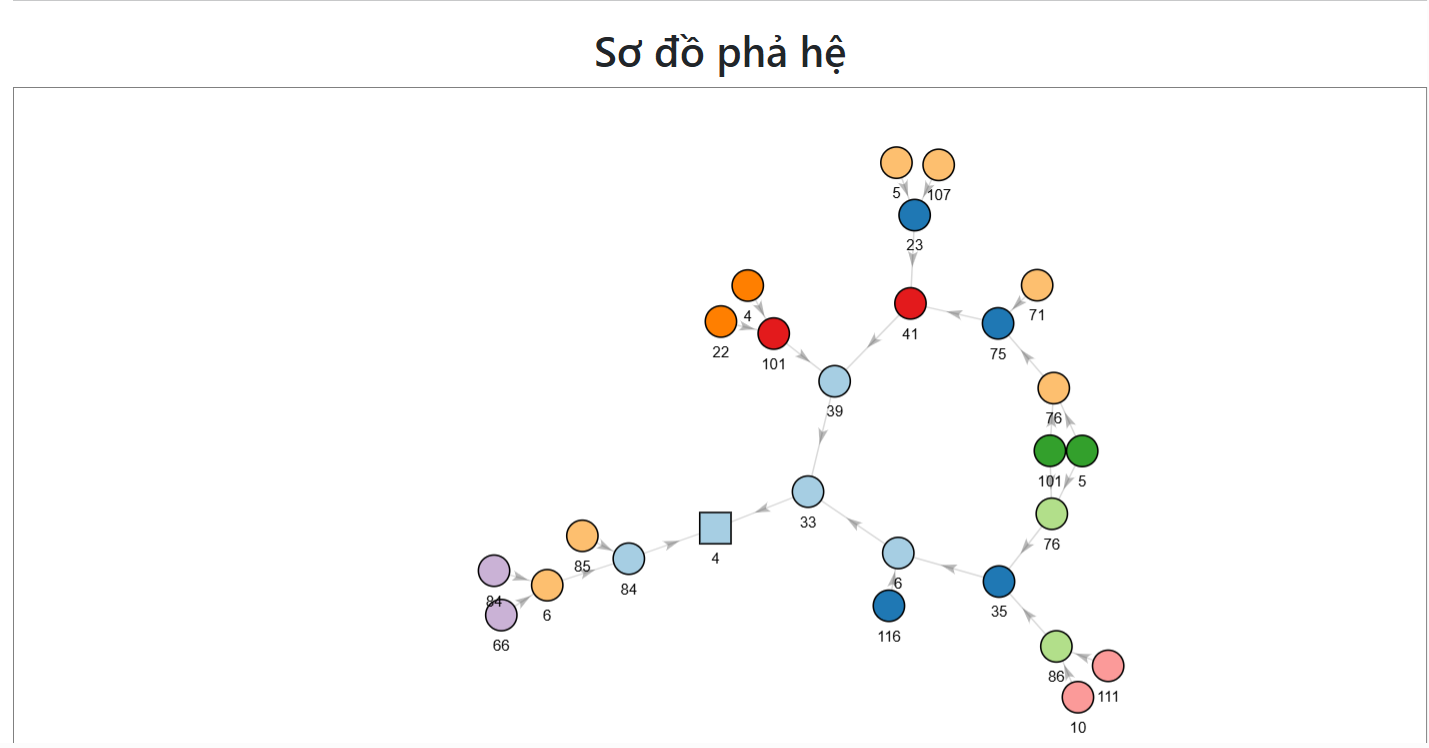
\includegraphics[scale=0.5]{figures/creature_relationship.png}
	\caption{Sơ đồ thế hệ kế thừa của một cá thể. Hình vuông thể hiện cá thể mục tiêu, mã màu khác nhau biểu thị cho thế hệ. Con số ghi dưới mỗi hình tượng trưng cho Id của cá thể.}
\end{figure}
